\section{Analysis strategy}\label{chap5:analysis_strategy}

\subsection{Event selection and objetc definition}

Regarding the electrons, muons, jets and \MET definition and reconstruction, the standard CMS recommendations described in Chapter~\ref{chap2} are used. The specific selections used in this analysis are briefly summarised below.

Muons are identified according to the CMS recommendations for the medium working point, with the addition of some extra cuts, as defined by the following selections:
\begin{itemize}
\item identified by the standard medium muon selection described in Sec.~\ref{sec:Objects}; \textcolor{red}{Not yet defined :)}
\item $\pt> 10$\GeV;
\item $|\eta < 2.4|$;
\item $|d_{xy}| < 0.01$\,cm for $\pt < 20$\GeV and $|d_{xy}| < 0.02$\,cm for $\pt > 20$\GeV, $d_{xy}$ being the transverse impact parameter with respect to the primary vertex;
\item $|d_{z}| < 0.1$\,cm, where $d_z$ is the longitudinal distance of the muon track in the tracker extrapolated along the beam direction.
\end{itemize}

For the muon isolation the CMS recommended particle flow isolation based on the tight working point is used, corresponding to a requirement on the isolation variable of $ISO_\mathrm{tight} < 0.15$. In addition a tracker relative isolation is also applied.

For the electron identification, the tight working point is used. In addition some additional cuts to make the selection ``trigger-safe'' are included. This is done because the electron triggers already include some identification and isolation requirements that are based on the raw detector information, while the offline selections make use of particle flow requirements. The ``trigger-safe'' selections are defined to make the the offline identification and isolation requirements tighter with respect to the online triggers.

The simulated events are corrected for the lepton trigger, identification and isolation efficiencies measured in data using the same techniques described in Sec.~\ref{sec:Selections}.

Jets are defined clustering the particle flow objects using the anti-$k_t$ algorithm with a distance parameter of 0.4. The CHS pileup mitigation technique is used. The L1, L2, L3 and L2L3 jet energy correction described in Sec.~\ref{sec:Objects} are applied. The reject jets coming from calorimeter or readout electronics noise, the loose working point for PF jet identification is used.

The b-tagging algorithm for this analysis is chosen comparing the performances of different algorithms using simulations for signal and background contributions in the phase space defined by the analysis kinematic requirements. More precisely, two MC samples are used, one corresponding the the \hwwllnn signal produced via the ggH production mode and another corresponding to the \ttbar process. In fact, the first sample is enriched in light jets, i.e. originating by the hadronization of light quarks like u,d,c and s quarks, while the second sample is enriched in b jets, coming from the top quark decay. The b-veto efficiency, $\epsilon_\mathrm{b veto}$, is computed separately for the two samples and for the various b tagging algorithms. To compare the b tagging performance $\epsilon_\mathrm{b veto}$ is computed for different working points, i.e. different selections on the specific b tagging discriminator, and the results are reported in the form of a ROC curve. The ROC curves corresponding to events with 0, 1 and $\geq 2$ jets are shown in Fig.~\ref{fig:btag}. Events considered for this study are the ones passing the WW baseline selection.

\begin{figure}[!h]
\centering
\subfigure[$N_\mathrm{jets} = 0$]{
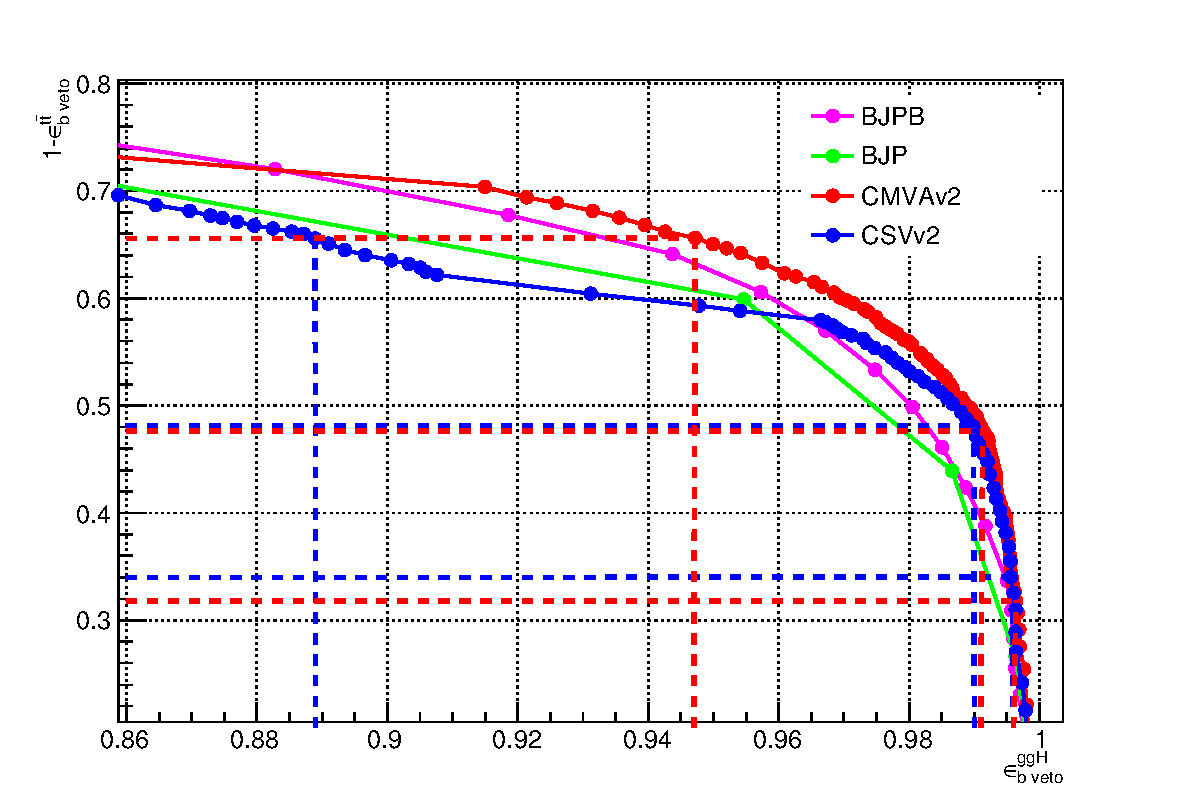
\includegraphics[width=0.45\textwidth]{images/13TeV/ROC_njet0.pdf}
}
\subfigure[$N_\mathrm{jets} = 1$]{
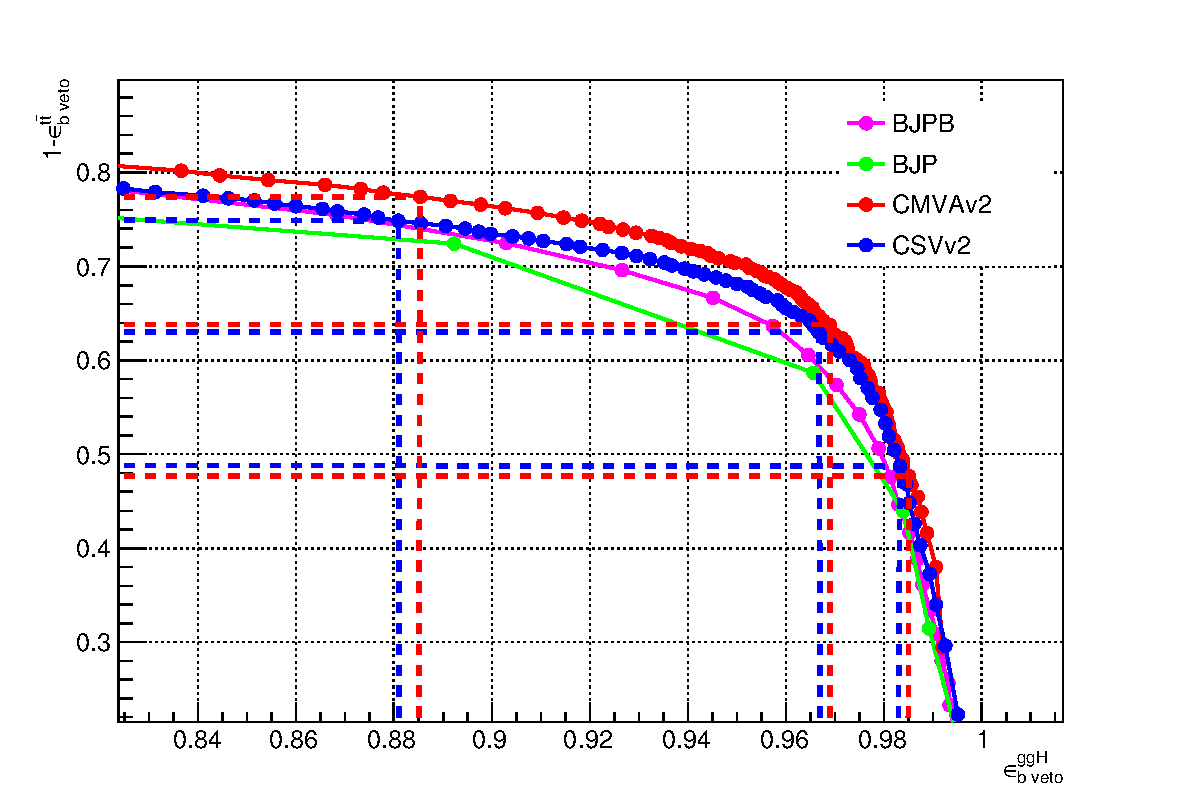
\includegraphics[width=0.45\textwidth]{images/13TeV/ROC_njet1.pdf}
}
\subfigure[$N_\mathrm{jets} \geq 2$]{
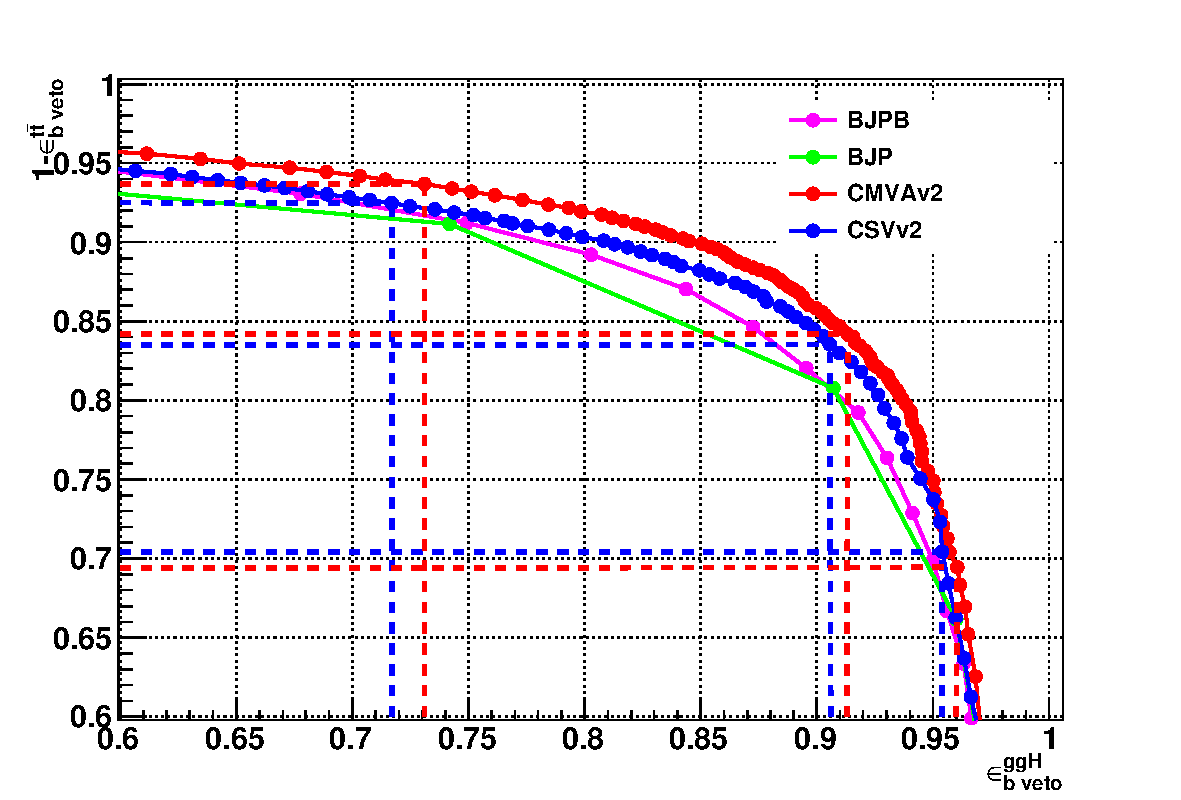
\includegraphics[width=0.45\textwidth]{images/13TeV/ROC_njetge2.pdf}
}
\caption{ROC curve for the b veto efficiency on signal and background events. The blue and red lines point out the signal efficiency and the background rejection corresponding to the three working points considered for the CSVv2 and the cMVAv2 algorithms
respectively.}\label{fig:btag}
\end{figure}

The ROC curves show that the cMVAv2 algorithm has the best performance for the analysis phase space among the algorithms taken into account. For both the CSVv2 and cMVAv2 algorithms, three working points are defined corresponding to the mistag rates\footnote{The mistag rate is defined as the probability for a light jet to be identified as a b-jet by the b tagging algorithms.} of 10\% for the loose, 1\% for the medium and 0.1\% for the tight working point. The distribution of the cMVAv2 discriminator associated to the leading jet both for the ggH and the \ttbar MC sample is shown in figure~\ref{fig:discriminator}.

\begin{figure}[!h]
\centering
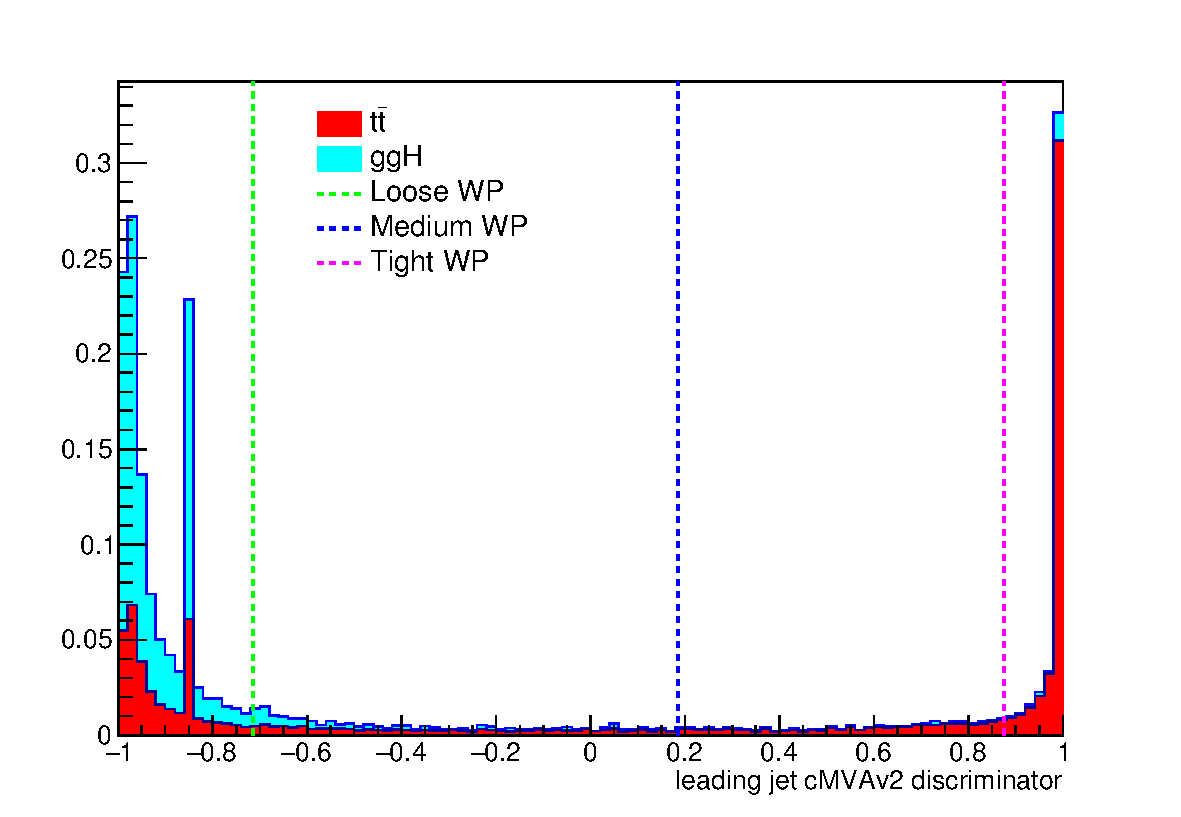
\includegraphics[width=0.8\textwidth]{images/13TeV/cmva_WP.pdf}
\caption{cMVAv2 discriminator associated to the leading jet (with $\pt > 30$~GeV) both for the ggH and the $t\bar t$ processes. The two processes are normalized to unity and stacked. The vertical dashed lines show the discriminator value corresponding to the three working points.}\label{fig:discriminator}
\end{figure}

In order to determine the best working point for this analysis a preliminary significance assessment is performed, using a complete analysis procedure in which only statistical
effects are taken into account (no systematics are included). The significance assessment
was performed using a two dimensional discriminating
variable consisting of the dilepton invariant mass versus the transverse
mass. The assessment was performed with the following leptonic selection:
\begin{itemize}
\item two leptons, an electron and a muon with opposite charge, with
leading lepton \pt greater than 20\GeV and sub-leading lepton \pt greater than
13\GeV;
\item no other lepton (electron or muon) with \pt greated than 10\GeV;
\item \mll greater than 12\GeV;
\item PF type 1 corrected MET greater than 20\GeV;
\item \ptll greater than 30\GeV.
\end{itemize}
In addition to this global selection, two categories were identified:
\begin{itemize}
\item 0 jets: no jets above 30\GeV, jets between 20\GeV and 30\GeV are
b-vetoed with the cMVAv2 WP under study;
\item 1 jet: exactly 1 jet above 30\GeV, no b-tagged jets above 30\GeV
according to the cMVAv2 WP under study.
\end{itemize}
The two categories were eventually combined together and the significance 
assessment was repeated for the three working points.
With these selection we find the significance values listed in
Table~\ref{tab:significance_wp_combine} for the three working points.
\begin{table}
\begin{center}
\begin{tabular}{cccc}
\toprule
Jet category & Loose WP (-0.715) & Medium WP (0.185) & Tight WP (0.875) \\
\midrule
0 jets & 2.022 & 2.043 & 2.036 \\
1 jet & 1.439 & 1.404 & 1.305 \\
$0+1$ jets & 2.481 & 2.479 & 2.420 \\
\bottomrule
\end{tabular}
\end{center}
\caption{Significance corresponding to the three working points and for
different jet categories using a shape
analysis.\label{tab:significance_wp_combine}}
\end{table}

The working point providing the best significance in the combined $0+1$ jets category is found to be the loose one.

To correct for a possible different b tagging efficiency in data and simulation, the simulated events are reweighted using scale factors computed in bins of the jet $\eta$ and \pt. These scale factors and the corresponding uncertainties are centrally calculated for each working point, in such a way to be employable by all the CMS analyses. The prescription to reweight the simulated events is the following. First of all one has to compute the b tagging efficiency using the MC samples, $\varepsilon_\mathrm{MC}(p_\mathrm{T}, \eta, f)$, for the chosen working point in bins of jet \pt and $\eta$. The efficiency has to be computed for different flavours $f$ of the jets, b, c and light (u,d,s), using the jet matching information\footnote{There are a couple of techniques developed by the CMS Collaboration to assess the flavour of a reconstructed jet in simulation. The technique used here makes use of the flavour of the hadrons clustered into a jet.} which is available in all the MC samples. An MC-based event weight is then calculated computing the probability $P_\mathrm{MC}$ of a given b tagging configuration to occur, e.g.:
\begin{equation}
P_\mathrm{MC}=\prod_{i~\in{}~b-tagged-jets}\varepsilon_{\mathrm{MC}_{i}}\prod_{j~\in{}~non-b-tagged-jets}(1-\varepsilon_{\mathrm{MC}_{j}})
\label{eq:btagpmc}
\end{equation}
Afterwards, a similar probability is computed using data:
\begin{equation}
P_\mathrm{DATA}=\prod_{i~\in{}~b-tagged-jets}SF_{i}\varepsilon_{\mathrm{MC}_{i}}\prod_{j~\in{}~non-b-tagged-jets}(1-SF_{j}\varepsilon_{\mathrm{MC}_{j}}) \quad ,
\label{eq:btagpdata}
\end{equation}
where $SF_{i}$ is the provided scale factor value for the relevant jet flavour, \pt and $\eta$. Products in Eqs.~\ref{eq:btagpmc} and \ref{eq:btagpdata} run over all jets. The event weight is finally given by the ration $P_\mathrm{DATA}/P_\mathrm{MC}$.

The b tagging efficiencies to be fed into Eq.~\ref{eq:btagpmc} and
Eq.~\ref{eq:btagpdata} are derived using \ttbar simulated events and applying basic leptonic
selections. These efficiencies are shown in Fig.~\ref{fig:effmc} for light
(a), c-jets (b) and b-jets (c), in bins of $\eta$ and \pt. The uncertainties associated to the efficiencies are representative of the statistics of the simulated \ttbar sample, and are computed according to a binomial distribution.
\begin{figure}[!h]
\centering
\subfigure[]{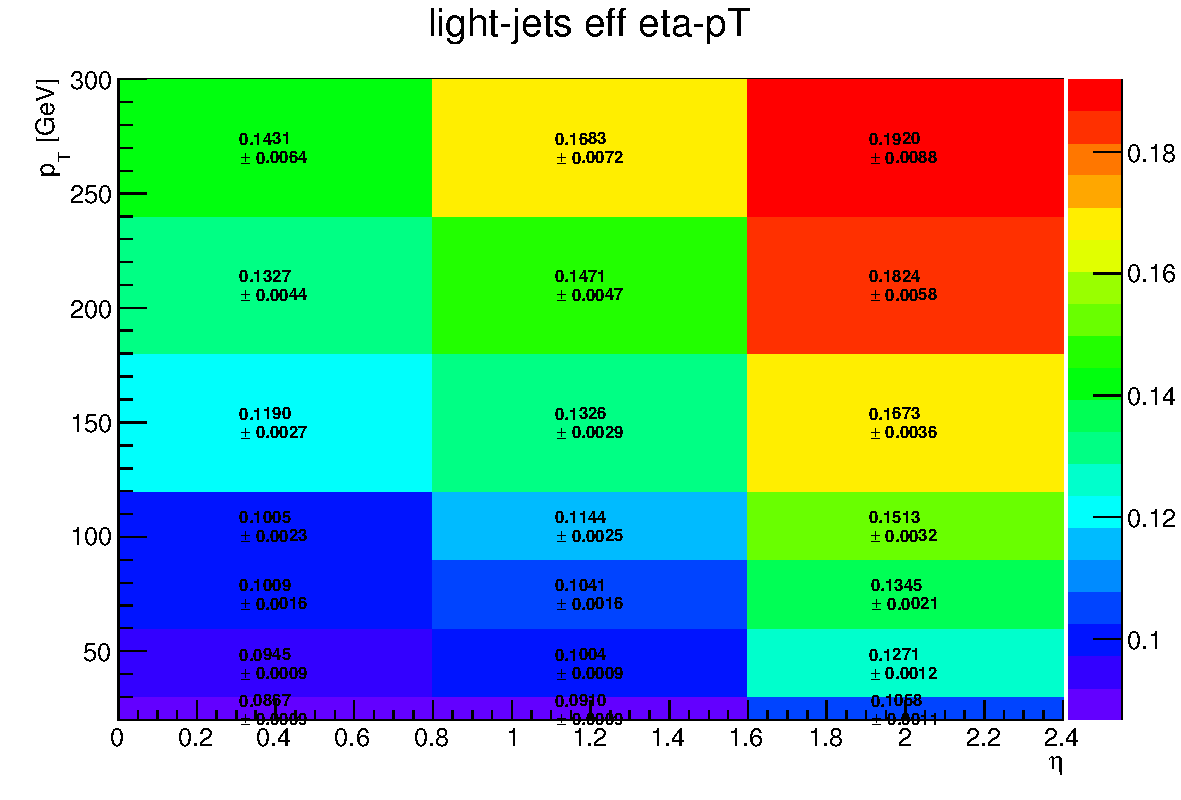
\includegraphics[width=0.4\textwidth]{images/13TeV/ljet_effmc.pdf}}
\subfigure[]{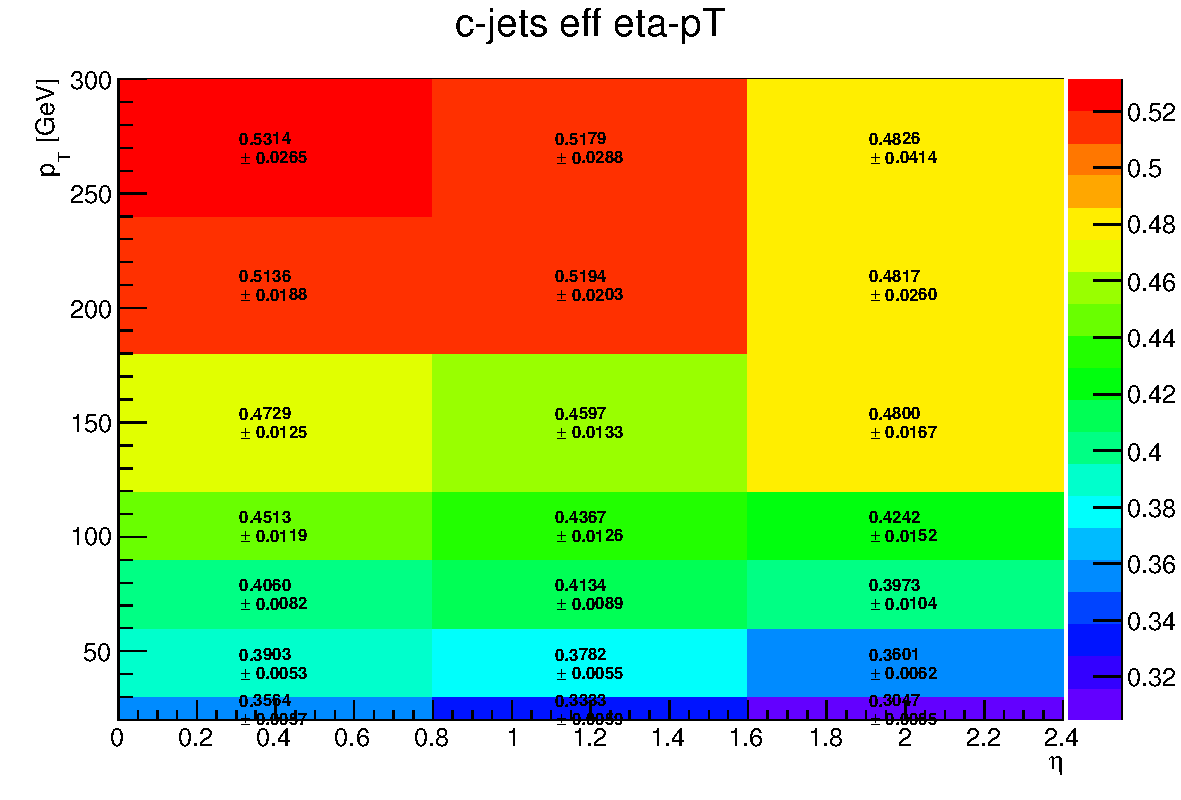
\includegraphics[width=0.4\textwidth]{images/13TeV/cjet_effmc.pdf}}\\
\subfigure[]{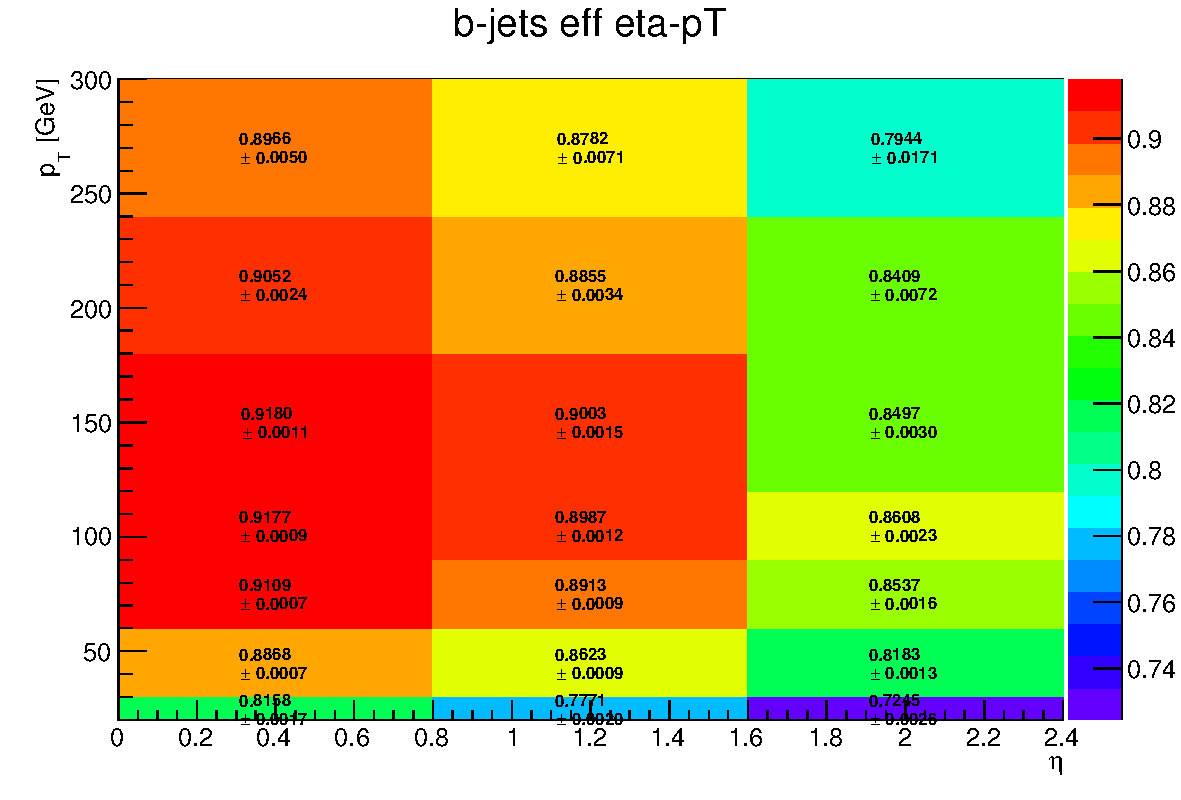
\includegraphics[width=0.4\textwidth]{images/13TeV/bjet_effmc.pdf}}
\caption{B tagging efficiencies for light jets (a), c-jets (b) and
b jets (c), as a function of $\eta$ and \pt.\label{fig:effmc}}
\end{figure}


The effect of the event reweighting is to correct the shape of the b tagging discriminator in simulation, moving events from the b tag region (discriminator greater than $> -0.715$) to the b veto region (discriminator $ < -0.715$) and viceversa. A data/simulation comparison of the b tagging discriminator for the leading and subleading jets is performed to check the agreement after the application of the event weights. In order to evaluate the data/simulation agreement for b-jets, the data and simulation are compared in a top enriched control region, defined by the following requirements:
\begin{itemize}
\item two leptons, an electron and a muon with opposite charge, with
leading lepton \pt greater than 20\GeV and sub-leading lepton \pt greater than
15\GeV;
\item no other lepton (electron or muon) with \pt greater than 10\GeV;
\item lepton invariant mass greater than 50\GeV;
\item at least two jets with \pt greater than 30 GeV;
\item at least one of the two leading jets with cMVAv2 btagging score
greater than -0.715 (i.e. the loose working point).
\end{itemize}
In order to evaluate the agreement for light jets, a second
control region is defined, populated by Z+light jet events, defined as follows:
\begin{itemize}
\item two leptons, two electrons or two muons with opposite charge, with
leading lepton \pt greater than 20\GeV and sub-leading lepton \pt greater than
15\GeV.
\item no other lepton (electron or muon) with \pt greater than 10\GeV.
\item lepton invariant mass greater between 80\GeV and 110\GeV.
\item at least two jets with \pt greater than 30 GeV.
\item at least one jet above 30\GeV.
\item no jets above 20\GeV with a TCHE score above 2.1. 
\end{itemize}
Although a Z+jets sample is dominated by light flavor jets, a b-veto on an
alternative algorithm (TCHE) is applied to reduce the contamination from b-jets,
especially above the cMVAv2 cut.  This helps mitigating possible data/simulation discrepancies in the modeling of the heavy/light flavor ratio.
The comparison between data and simulation after the event reweighting is shown in Figs.~\ref{fig:bpogSF} and \ref{fig:bpogSF_Z} for the b-jets and light jets enriched control regions, respectively.

\begin{figure}[!h]
\centering
\subfigure[]{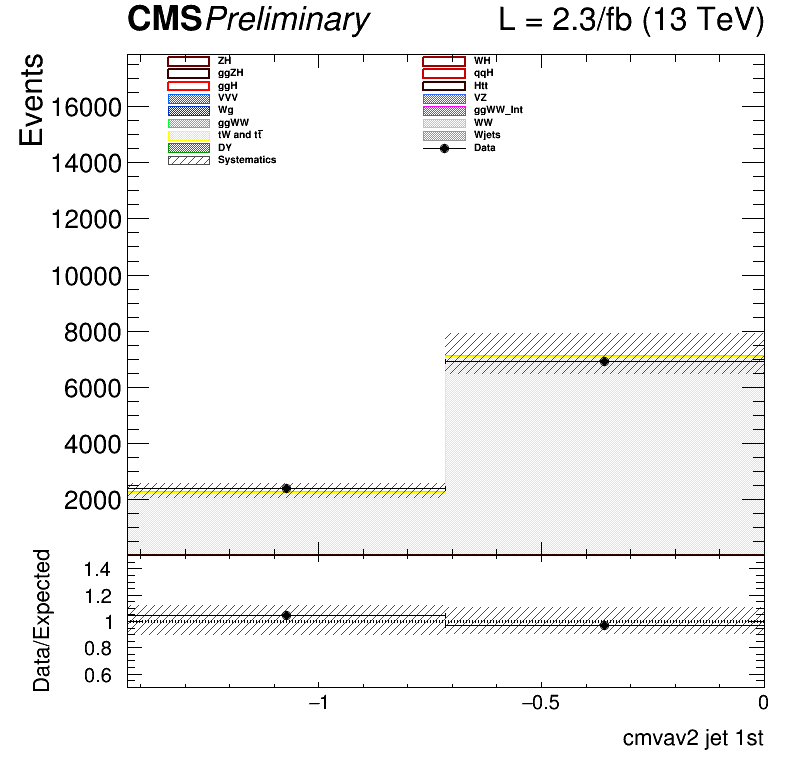
\includegraphics[width=0.4\textwidth]{images/13TeV/cratio_hww2l2v_13TeV_top_of1j_cmva_twobins_1.png}}
\subfigure[]{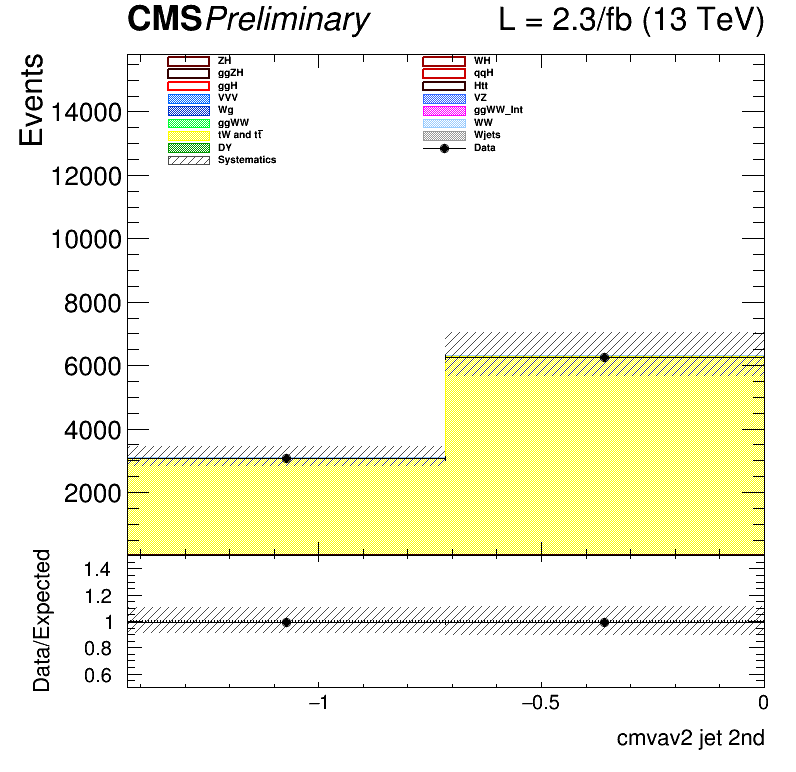
\includegraphics[width=0.4\textwidth]{images/13TeV/cratio_hww2l2v_13TeV_top_of1j_cmva_twobins_2.png}}
\caption{B tagging cMVAv2 discriminator for the leading (a) and the subleading (b)
jet in the b-jets enriched control region.\label{fig:bpogSF}}
\end{figure}
\begin{figure}[!h]
\centering
\subfigure[]{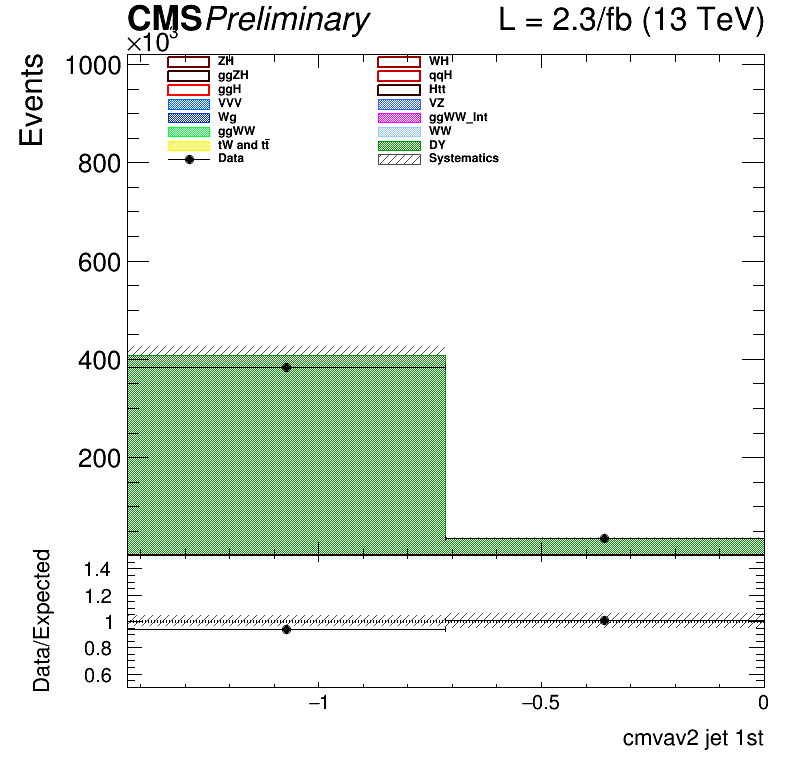
\includegraphics[width=0.4\textwidth]{images/13TeV/cratio_ZjetsCutTCHE_mumu_cmva_twobins_1.png}}
\subfigure[]{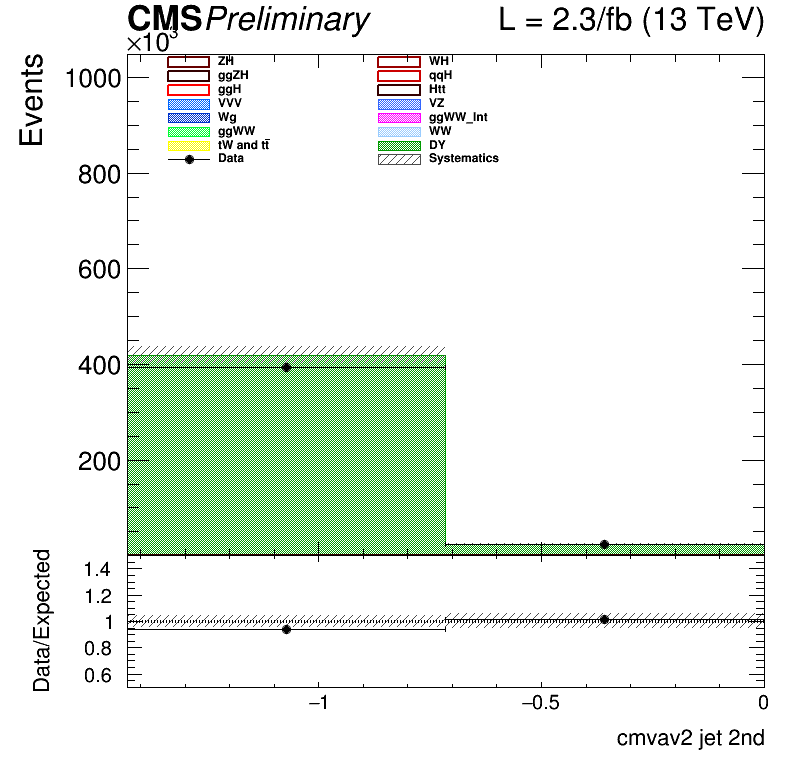
\includegraphics[width=0.4\textwidth]{images/13TeV/cratio_ZjetsCutTCHE_mumu_cmva_twobins_2.png}}
\caption{B tagging cMVAv2 discriminator for the leading (a) and the subleading (b)
jet in the light jets enriched control region.\label{fig:bpogSF_Z}}
\end{figure}
